%-------------------------------------------------------------------------------
\section{Case Studies}
%-------------------------------------------------------------------------------
\label{sec:hotcrp_example}

\iffalse
\begin{figure}[t!]
    \centering
    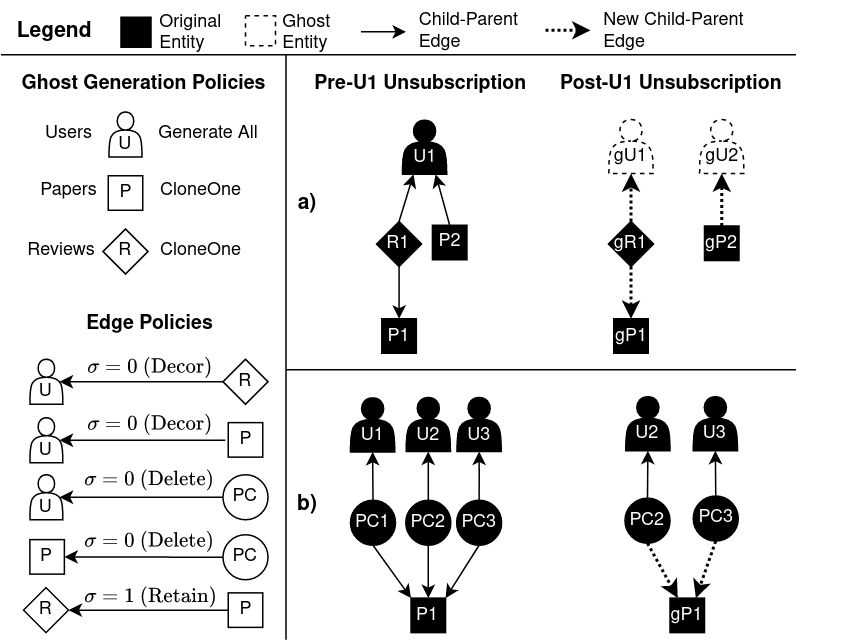
\includegraphics[width=.55\textwidth]{img/decor_hotcrp}
\begin{lstlisting}[language=Rust]
"User-Review":  Retain
"User-Paper":   Retain
"Review-Paper": Retain
\end{lstlisting}

\begin{lstlisting}[language=Rust]
"User-PaperConflict":  Delete
"PaperConflict-Paper": Delete
\end{lstlisting}
    \caption{Effects of the HotCRP-Granular unsubscription disguise. We show
    only relevant parts of the object graph and disguise.\\
    }
    \label{fig:hotcrp}
\end{figure}
\fi

\begin{table}[t!]
    \centering
    \footnotesize
    \begin{tabular}{@{}ccccc@{}}
        \multirow{2}{*}{\textbf{App}} & \textbf{\#Object} & \textbf{\#Edge} & \textbf{Schema} &
        \textbf{Disguise} \\
        & \textbf{Types} & \textbf{Types} & \textbf{LoC} & \textbf{LoC} \\
    \midrule
    Lobsters-Current & 19 & 20 & 318 & 220 \\
    HotCRP-Current & 25 & 50 & 352 & 378 \\
    HotCRP-Granular & 25 & 50 & 352 & 407 \\
\end{tabular}
    \caption{Data disguise specifications for Lobsters and HotCRP have similar complexity to
    a relational schema.
    %Lobsters retains and reassigns user contributions to an anonymous user, and HotCRP deletes
    %direct correlations to the user.
    }
\label{tab:loc}
\end{table}
We evaluate whether \sys enables developers to easily express and automate practical data disguises
by writing disguises for user account deletion in Lobsters, an open-source news feed application, and
HotCRP, an application for conference review management. Writing disguises should be of similar
difficulty and require the same expertise as writing relational schemas. In particular, a developer
should write a disguise only once. Because disguises require at most one transformation for
each object type and edge type, disguise complexity is limited by the number of entity types and
relations in the application schema. Table~\ref{tab:loc} shows the statistics for each disguise.

%We next describe HotCRP unsubscription disguises in more detail. HotCRP objects include users
%(reviewers and authors), papers, paper reviews, and paper conflicts.  Users who unsubscribe are
%mainly concerned with deidentifying their identity from their reviews and authored papers: someone
%%with access to those papers or reviews should not be able to reassociate these papers or reviews
%with the unsubscribed user.

Lobsters-Current and HotCRP-Current implement the current account deletion policies in the respective
applications.
%The HotCRP-Coarse disguise specifies the current HotCRP unsubscription policy, which deletes all
%objects correlated to the user.
%simply deletes users' reviews, paper conflicts, and other review information. HotCRP-Coarse specifies
%\texttt{Delete} edge transformations for edge types to the user, and \texttt{Retain} for all other
%edges.
%
%All sensitive objects are either removed or retained, and no guises are
%generated. HotCRP-Coarse there does not explicitly specify any object transformations.
%
%Each of the 50 edge transformation specifications requires 6LoC, and the remaining 78 LoC of the disguise
%definition come from defining \sys data structures for a total of 378 LoC.
%
HotCRP-Granular specifies a HotCRP account deletion policy that balances useful data
retention with data deletion for privacy, as described in \S\ref{design:eg}.
%HotCRP-Granular keeps reviews and review metadata present
%for other users to use.
%
%Instead of deleting a user's papers, reviews, and paper conflicts, HotCRP-Granular specifies
%to \texttt{Decorrelate} edges from users to reviews and papers. This retains paper and
%reviews, but decorrelates them from the user: \sys replaces these edges with an ones to generated
%ghost user profiles.
%
%A paper's set of paper conflicts can also identify unsubscribed users by exposing their affiliations and recent
%collaborations. HotCRP-Granular \texttt{Delete}s paper-to-paper conflict edge types, removing all
%edges from the user's paper conflicts to papers.
%%
%Deleting conflicts can lead to spurious conflicts (\eg no coauthor is affiliated with NYU, but NYU
%reviewers have conflicts), but does not break HotCRP's paper visibility or review assignment
%invariants.
%A more complete de-identification would to delete \emph{all} the paper's
%conflicts, but incorrectly allows users with reviewer conflicts to review a paper and
%break HotCRP semantics.
%
%HotCRP-Granular \texttt{Retain}s all other edge types. This ensures that review and paper artifacts
%remain correctly linked: (subscribed) reviewers still see the correct paper for their reviews, and
%(subscribed) authors see the correct reviews for their papers.
%
%Users are linked to papers via \emph{paper conflict} entities, which have both a user and a paper
%as a parent, and indicate either a collaborator, or a reviewer conflict (prior collaborators or
%sharing an institution).
%Thus, correlations from the user's papers to paper conflicts should be broken: we specify
%, and review and paper metadata should remain correctly associated.
%
%HotCRP-Granular transforms users into guises to decorrelate reviews and papers from the
%user by generating default or suitable random attribute values
%(\eg timestamps randomly generated within the past decade). In particular,
%\texttt{disabled} is set to \texttt{true}, ensuring that guises have no permissions and never review papers.
%Paper and review objects are copied to retain their information.
%%This results in a slightly longer, 407 LoC disguise specification.
%We copy all paper and review attributes once, retaining paper and review information without creating duplicates.
%and clones paper conflicts because no conflict
%value attributes are identifying.

%\textbf{Lobsters} has a total of 20 entities, and a \lyt{TODO} LoC mask specification for unsubscription.
%The mask replicates what the behavior of the current Lobsters deployment upon user unsubscription,
%with the exception that we replace users with ghost users rather than a global placeholder, and we
%desensitize tags so that sensitive stories comprise at most 25\% the number of stories with a
%particular tag. This limits how much a particular tag topic can be used to identify a user who often
%posts about that topic (e.g.,\ a researcher in visualization).
%We decorrelate all edges directly to the user, and edges from sensitive stories to tags will
%decorrelate to a sensitivity threshold of 0.25 (with ghost tags generated as a default tag).
%We retain all other types of edges.

\subsection{Performance Challenges}
\label{sec:perf}

\begin{figure}[t!]
    \centerline{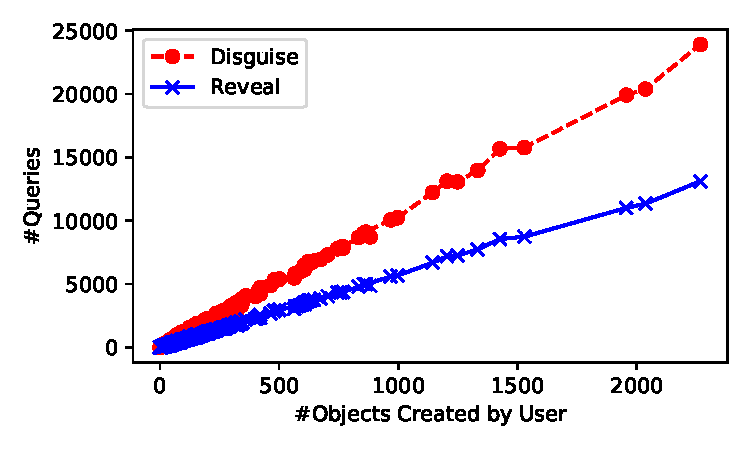
\includegraphics[width=.5\textwidth]{img/perf}}
    \caption{Number of queries required by Lobsters-Current to disguise and reveal a target user, depending on the number of
    objects created by the user.}
    \label{fig:latencies}
    \vspace{-\baselineskip}
\end{figure}

Our experience implementing \sys exposed the challenging performance tradeoff between efficiently
executing normal application queries, and achieving low-latency disguise application. The right
balance depends on the rate of disguising, which may range from rare (as in today's applications),
to quite frequent in a privacy-supporting world where users freely disguise and reveal themselves,
or where data automatically ages out.
%\sys incurs overheads from adding a layer of indirection between application and database, and
%applying disguises (\eg creating guises).
%We implemented several \sys variants to explore different performance tradeoffs.

One \sys variant adds minimal normal execution overhead, only intercepting application queries; this
decreases throughput by 4\% compared to a baseline without \sys. Another variant additionally
tracks an in-memory object graph, decreasing throughput by 9\% compared to baseline.
%
Worst-case disguise application creates as many guises as the number of edges connected to the
target. Figure~\ref{fig:latencies} depicts how many SQL queries \sys performs while disguising and
revealing users. \sys applies the Lobsters-Current disguise in an object graph with 3K users and 80K
total user contributions. Disguising currently performs queries sequentially during object graph
traversal; revealing batches queries by table. Queries increase linearly with the number of objects
created by the target user.

This indicates a need for privacy-aware database designs, which spread the cost of disguising across
normal execution.
%
One possibility keeps a ``shadow'' copy of the database that reflects the disguised state, with
guises already created and edges rewritten.
%
Pre-created guises are hidden by transparently exposing materialized views (MV) to the application.
Disguising simply exposes the shadow copy in the MV, and removes objects that should be deleted.
%
This achieves good read performance---queries read from MVs instead of the database---albeit with
high memory consumption. However, normal execution write queries now must potentially update
multiple guises in the shadow copy, and
pre-created guises consume space during normal execution, even if disguises are never applied.
%
Other possibilities include making disguises eventually consistent; updating the shadow copy
asynchronously; and caching disguises for users who are disguised (and revealed) most often.
%and using dataflow to more efficiently update materialized views when disguising.

%%%%%%%%%%%%%%%%%%%%%%%%%%%%%%%%%%%%%%%%%%%%%%%%%%%%%%%%%%%%%%%%%%%%%%%%%%%%%%%%%%%%%%%%%
\iffalse
\begin{figure}[t!]
    \centering
    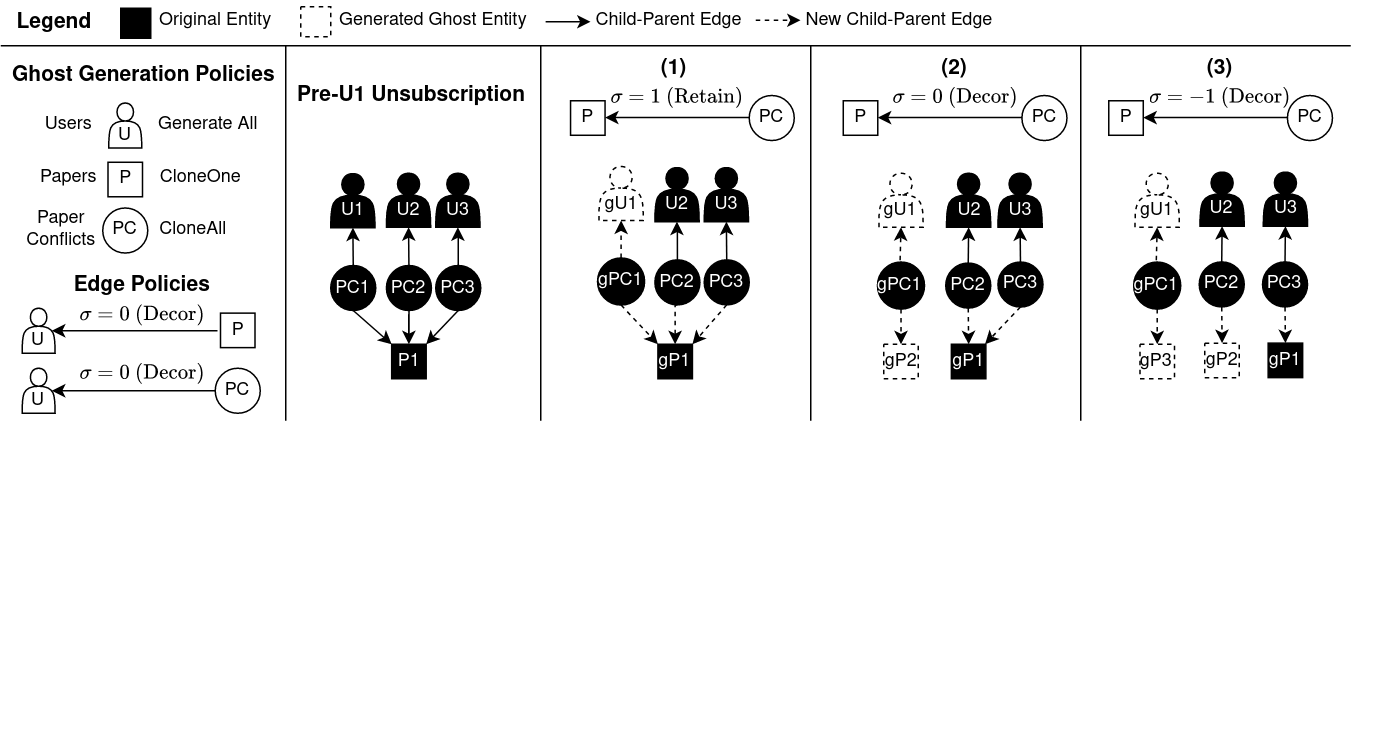
\includegraphics[width=.5\textwidth]{img/pcs}

    \caption{Potential edge policies for paper-conflict to paper edges in HotCRP.
    (1) retains edges from sensitive conflicts to papers; (2) decorrelates sensitive
    conflicts from papers; (3) decorrelates all conflicts from papers.
    In (3), a negative sensitive threshold causes \sys to
decorrelate \emph{all} children, including non-sensitive ones.}
    \label{fig:pcs}
\end{figure}

Here, the developer can make one of three choices.
These choices demonstrate the tradeoff between retaining information for application correctness, and completely de-identifying the user.
Figure~\ref{fig:pcs} shows the post-unsubscription application state resulting from each choice.
%
(1) retains correlations between sensitive paper conflicts and papers, at the cost of
user privacy; (2) decorrelates sensitive paper conflicts from the paper so each
sensitive paper conflict is reassociated with a ghost paper parent, but can lead to spurious,
unexplained conflicts; and (3) decorrelates \emph{all} paper conflicts correlations
with the paper, but breaks HotCRP paper visibility semantics.
While no choice is perfect, we choose policy 2, shown in Figure~\ref{fig:hotcrp}b, which provides
stronger user privacy and acceptable semantics for HotCRP.
%If the user resubscribes, the decorrelated paper conflict is
%relinked to the user and the original paper, restoring the original state. If all users with
%conflicts to the same paper decorrelate, the paper will have no associated paper conflicts.

%The first choice retains correlations between sensitive paper conflicts and papers. This allows
%other users to see that some ghost user has a conflict with the paper, and potentially
%derive the user's identity by deducing the users' affiliation or collaborators based on the paper
%conflicts between the paper and other users.
%
%The second choice decorrelates sensitive paper conflicts from the paper with a sensitivity threshold
%of 0. This ensures that each sensitive paper conflict will be associated with a ghost paper parent
%after unsubscription. To other users who can view the paper, it will appear as the sensitive paper
%conflict never existed. Unlike the first choice, this can lead to spurious, unexplained conflicts:
%for example, the PC may observe that a reviewer who works at BU has a conflict with a paper, but
%none of the paper's authors are from BU (because the author unsubscribed, and their conflict was
%decorrelated from the paper). Spurious conflicts can lead to identifying information leakage: in
%this case, observers can see at least one unsubscribed user likely works at BU. However, unlike the
%first choice, other users cannot be sure of exactly how many unsubscribed users and conflicts
%initially existed, and if no spurious conflicts are produced, cannot deduce that an unsubscribed
%user had a conflict at all. In addition, if the unsubscribed user had a reviewer conflict instead of
%a author conflict with the paper, then this choice leaks no identifying information at all.
%
%The third choice decorrelates \emph{all} paper conflicts correlations with the paper. While this
%certainly removes all potentially identifying information derivable from paper conflicts, this
%breaks HotCRP semantics: users who should not be able to view the paper (due to conflicts) will
%suddenly be able to.

%The HotCRP developer may also determine that tags can identify a user if only that user's papers are
%associated with that tag. The developer thus specifies that paper-tag edges have a sensitivity
%threshold of 0.5: at most half the papers with that tag can be associated with the unsubscribing
%user. \sys decorrelates these edges until the threshold is met; all ghost tag attributes are
%generated using a clone-one ghosting policy.  Figure~\ref{fig:hotcrp}c shows how \sys partially
%decorrelates a user's papers from a shared tag parent.
%\lyt{I know this doesn't exactly reflect HotCRP's schema (which uses PaperTags to link papers to
%tags), but I found this example the most convincing to demonstrate partial decorrelation. This may
%be more relevant in a different application than HotCRP.}

%\paragraph{Generating Ghost Entities.}
The developer also specifies how \sys generates ghost entities. The developer determines which entity
attributes reveal identifying information (and should be generated); which attributes should be
cloned to retain information necessary to the application; and how to generate attribute values in
ways that satisfy HotCRP semantics.
%If ghost entities cannot be generated without breaking
%application semantics, the relevant edges should be deleted instead of decorrelated.
For simplicity, Figure~\ref{fig:hotcrp} shows entity-granularity ghosting policies rather than
per-attribute ghosting policies.
%, and does not display the generation method (\eg random, default, etc.).
\sys generates ghost users' attributes, giving all ghosts a default value of \texttt{disabled=true}
to ensure ghosts never review papers. \sys clones all paper and review attributes once, retaining
paper and review information without creating duplicates, and clones paper conflicts because no conflict
value attributes are identifying.

%The developer may choose to
%clone attributes such as the user's roles once, to ensure that the number of users with a certain
%role does not change.

%In particular, it is safe to clone edges to user parents because the developer knows that \sys will
%decorrelate edges to sensitive parents (replacing them with edges to ghost parents) \emph{prior} to
%ghosting the child entity (the paper). Thus, any cloned edge attributes will necessarily point to
%ghosts if there was a sensitive correlation between the paper and user parent.  We see a concrete
%example of this in Figure~\ref{fig:algo}: step 3b ensures that the user and tag parents or any
%sensitive papers are appropriately ghosted prior to step 4, which ghosts the paper.
%
%Finally, the developer specifies a ghost generation policy for paper conflicts. Paper conflicts have
%three attributes, a value attribute for the conflict type (authorship or reviewer conflict), and two
%edge attributes that specify a user parent and a paper parent respectively. The developer defaults
%conflict type attributes to be \texttt{ConflictAuthor}, and clones the two edge attributes for all
%ghosts; edge policies ensure that cloned edges will point to ghosts if there was a sensitive correlation between
%the paper conflict and its original parents.
%As with paper entities, it is safe to clone edges to user and paper parents because any
%cloned edge attributes will necessarily point to ghosts if there was a sensitive correlation between
%the paper conflict and its parents.

%Note that had the developer chosen edge policy choice 1 for paper-conflict to paper edges
%(retaining the edge), then the conflict type \emph{must} be cloned in order to preserve HotCRP
%semantics. If the conflict type were a reviewer conflict, but the ghost paper conflict defaulted to an
%authorship conflict, this would cause HotCRP to report an extra author when one does not exist.
%With policy choice 2, both the user and paper parents are generated ghosts, and the conflict type is
%irrelevant to HotCRP.
%

%%%%%%%%%%%%%%%%%%%%%%%%%%%%%%%%%%%%%%%%%%%%%%%%%%%%%%%%%%%%%%%%%%%%%%%%%%%%%%%%%%%%%%%%%%%%%%%%%%%%%%
%%%%%%%%%%%%%%%%%%%%%%%%%%%%%%%%%%%%%%%%%%%%%%%%%%%%%%%%%%%%%%%%%%%%%%%%%%%%%%%%%%%%%%%%%%%%%%%%%%%%%%
%%%%%%%%%%%%%%%%%%%%%%%%%%%%%%%%%%%%%%%%%%%%%%%%%%%%%%%%%%%%%%%%%%%%%%%%%%%%%%%%%%%%%%%%%%%%%%%%%%%%%%
%%%%%%%%%%%%%%%%%%%%%%%%%%%%%%%%%%%%%%%%%%%%%%%%%%%%%%%%%%%%%%%%%%%%%%%%%%%%%%%%%%%%%%%%%%%%%%%%%%%%%%
We evaluate \sys on two metrics: (1) can desired decorrelation policies be easily specified using the
provided decorrelation primitives for a range of practical applications?, and (2) can decorrelation
be supported with low performance overhead?

Our evaluation exemplifies how a suite of applications can express a diverse
range of privacy policies using \sys with low developer effort with low overhead.

\subsection{Example policies}
\begin{figure}
\begin{lstlisting}[language=Rust]
use GhostColumnPolicy, GeneratePolicy;
let ghost_policies = GhostGenerationPolicy::new(
  ("users",
     [("id", Generate(Random)),
     ("username", Generate(Random)),
     ("karma", Generate(Default(0)))]),
  ...);

let edge_policies = vec![
  KeyRelationship{
    child: "stories".to_string(),
    parent: "users".to_string(),
    column_name: "user_id".to_string(),
    parent_child_decorrelation_policy: Decor,
    child_parent_decorrelation_policy: NoDecorRetain,
  },
  KeyRelationship{
    child: "taggings".to_string(),
    parent: "tags".to_string(),
    column_name: "tag_id".to_string(),
    parent_child_decorrelation_policy:
        NoDecorSensitivity(0.25),
    child_parent_decorrelation_policy: NoDecorRetain,
  },
  ...];

 ApplicationPolicy {
    entity_type_to_decorrelate: "users",
    ghost_policies: ghost_policies,
    edge_policies: edge_policies,
 }
\end{lstlisting}
    \label{fig:lobsters_policy}
    \caption{Excerpt of the Lobsters Application Policy}
\end{figure}
We provide several variants of an application policy for Lobsters, as well as example policies for a
HotCRP, software for conference reviews, and PrestaShop, an
open-source e-commerce web application.

\paragraph{Lobsters}
Lobsters has a total of 20 entities, and
these Lobsters policies require specifying at most 17 key
relationships and at most 5 ghost entity generation policies (see Figure~\ref{fig:lobsters_policy} for an example
of these policy specifications).

The first policy replicates what the behavior of the current Lobsters deployment upon user
unsubscription, with the exception that users are replaced with ghost users rather than a global
placeholder. This requires specifying \texttt{Decorrelate} policies for all edges from entities with users
as parents, resulting in the developer writing 9 edge policies and one ghost generation policy (for
ghost users). While this policy does nothing significant, splitting a user into multiple ghosts as
compared to a global placeholder allows the user to resubscribe by identifying their ghost
counterparts, whereas a global placeholder does not. Furthermore, splitting users into multiple
users as compared to grouping them together upon unsubscription may benefit privacy: global
placeholder users indicate that any child of the placeholder belongs to some deleted user, whereas
ghost users may more successfully mask which children have been abandoned.

The second policy decorrelates all user-related edges, but additionally desensitizes tags so the
taggings associated with sensitive stories are at most 25\% the number of stories with that tag.
Ghost stories clone randomly chosen existing stories with slight variations on the url.
This limits the amount that an observer can determine that a particular story was posted by a
particular user simply by knowing that a certain user has posted about the tag topic (e.g.,\ a researcher
in visualization). However, Lobsters still retains the content of these tagged stories.

\lyt{TODO} third policy.

\paragraph{HotCRP.}
HotCRP entities include users (reviewers and paper authors), papers, and paper reviews. There are a total of 25
entities, with 48 foreign key relationships between entities.
%; specifying these key relationships (as a non-maintainer of the HotCRP site) required x hours

HotCRP's current privacy policy~\cite{hotcrp:privacy} allows site managers (e.g.,\ program chairs)
to indefinitely store and distribute submissions and reviews. Each HotCRP.com user has an associated
global profile and a profile for every HotCRP.com site, and must contact the HotCRP maintainers
directly to remove these profiles. This corresponds to key relationships with
\texttt{NoDecor:Retain} policies: a user simply cannot unsubscribe (or resubscribe).

With \sys, we can express better, more granular privacy policies that would otherwise be difficult to
implement right in HotCRP. First, we specify that the top-level entity to decorrelate is a user
(entities of the \texttt{ContactInfo} table). These include reviewers who may want
to remove their connections with their reviews, papers, and other metadata (such as papers they
have requested to review).
Because all the entities such as reviews, papers, and review requests linked to unsubscribed users
may leak the user's identity, we then mark parent-child edges with the user as parent with a
\texttt{Decorrelate} policy, replacing the user with a ghost user profile. This goes beyond
pseudonymization: the user's reviews or papers are no longer grouped together by any (even anonymized)
identity. Ghost profiles are generated randomly.

We next observe that edges that are not directly linked to the user may also reveal identifying
information about the user's identity: the group of collaborators or conflicting members of the PC
may pinpoint the identity of the ``ghost user'' on a paper. Users are linked to papers via
\emph{paper conflict} entities, which have both a user and a paper as a parent. When a user
unsubscribes, our policy decorrelates the user from their child paper conflict entity.

To ensure that this sensitive conflict is not also correlated with a group of collaborators or conflicting PC
members, which might potentially identify the ghost user, we mark the (child-parent) edge from
the paper conflict to the paper with a \texttt{Decorrelate} policy. This replaces the paper conflict's
paper with a ghost paper.
To other users who can view the paper, it will appear as if the unsubscribing
user never had a paper conflict with the paper.
If the user resubscribes, the decorrelated paper conflict is relinked to the user and the original
paper, restoring the original state.  If all users with conflicts to the same paper decorrelate, the
paper will seemingly have no associated user accounts.

Ghost papers are generated using a \texttt{CloneOne} policy: all of the ghost papers generated are
set to some default template paper except for the ghost paper generated when the decorrelating
conflict is the \emph{last} conflict linked to the paper. This last ghost paper is generated as a
clone of the original paper, allowing HotCRP to retain information about the paper and
non-user-related paper metadata in the system.
\lyt{I believe it might be incorrect to create all ghost papers as clones of the original (with
different IDs, of course) because this would interfere with other paper attributes queried by the
system (tags, topics, etc.)?}

The final part of our policy ensures that review and paper artifacts remain present and
correctly linked with other application entities: (subscribed) reviewers should still see the correct paper for each of
their reviews, (subscribed) authors should see the correct reviews for their papers, and review and
paper metadata should remain correctly associated. We specify
\texttt{NoDecor:Retain} policies for all edges that were not assigned a policy in the prior
steps.

\paragraph{PrestaShop.}
PrestaShop entities include customers, products, orders, carriers, employees, and shops (as well as
many other entities such as product categories, languages, countries, shopping cart, etc.) There are
214 total different entities.

Due to the large scope of the schema, we automatically generate policies for the 324 key relationships between them
with \texttt{NoDecorrelation:Retain} policies, which means that \sys does, by default, no work upon
decorrelation and recorrelation. (We could also imagine that a \texttt{Decorrelate} or
\texttt{NoDecorrelate:Remove} policy could be
the default here, but we choose a policy by default that will not break application semantics,
instead of a policy that provides the strongest possible unsubscription privacy).

By simply providing a ghost customer generation policy and modifying all key relationships with
customer parents to \texttt{Decorrelate} or \texttt{Remove} policies, PrestaShop can ensure that
customer information is appropriately de-identified when a customer unsubscribes.
Currently, PrestaShop has explicit GDPR policies for its merchants when a customer requests to delete
their account: their personal account details (age, email, address) are removed, but order invoices
and abandoned carts are transferred to an anonymous account
\lyt{TODO \url{https://doc.prestashop.com/display/PS17/Complying+with+the+GDPR}}.
\sys allows PrestaShop to go beyond pseudonymity, creating individual (ghost) accounts for each
cart and order invoices of a customer, and also allowing a customer to retrieve these orders and
abandoned carts if she rejoins the application.

\sys also can help PrestaShop keep attributes such as the country or language of a user for
statistical analyses (used by merchants to analyze product popularity). Ghost customers can generate
links to countries nearby a set of countries similar to the original user; if this still reveals too
much sensitive information, the location can be desensitized (adding additional generated ghost
customers not related to the original user for noise).

This process requires going through each of the individual key relationships, which must be done to
generate the schema in the first place.

\subsection{Performance}

\begin{figure*}[h!]
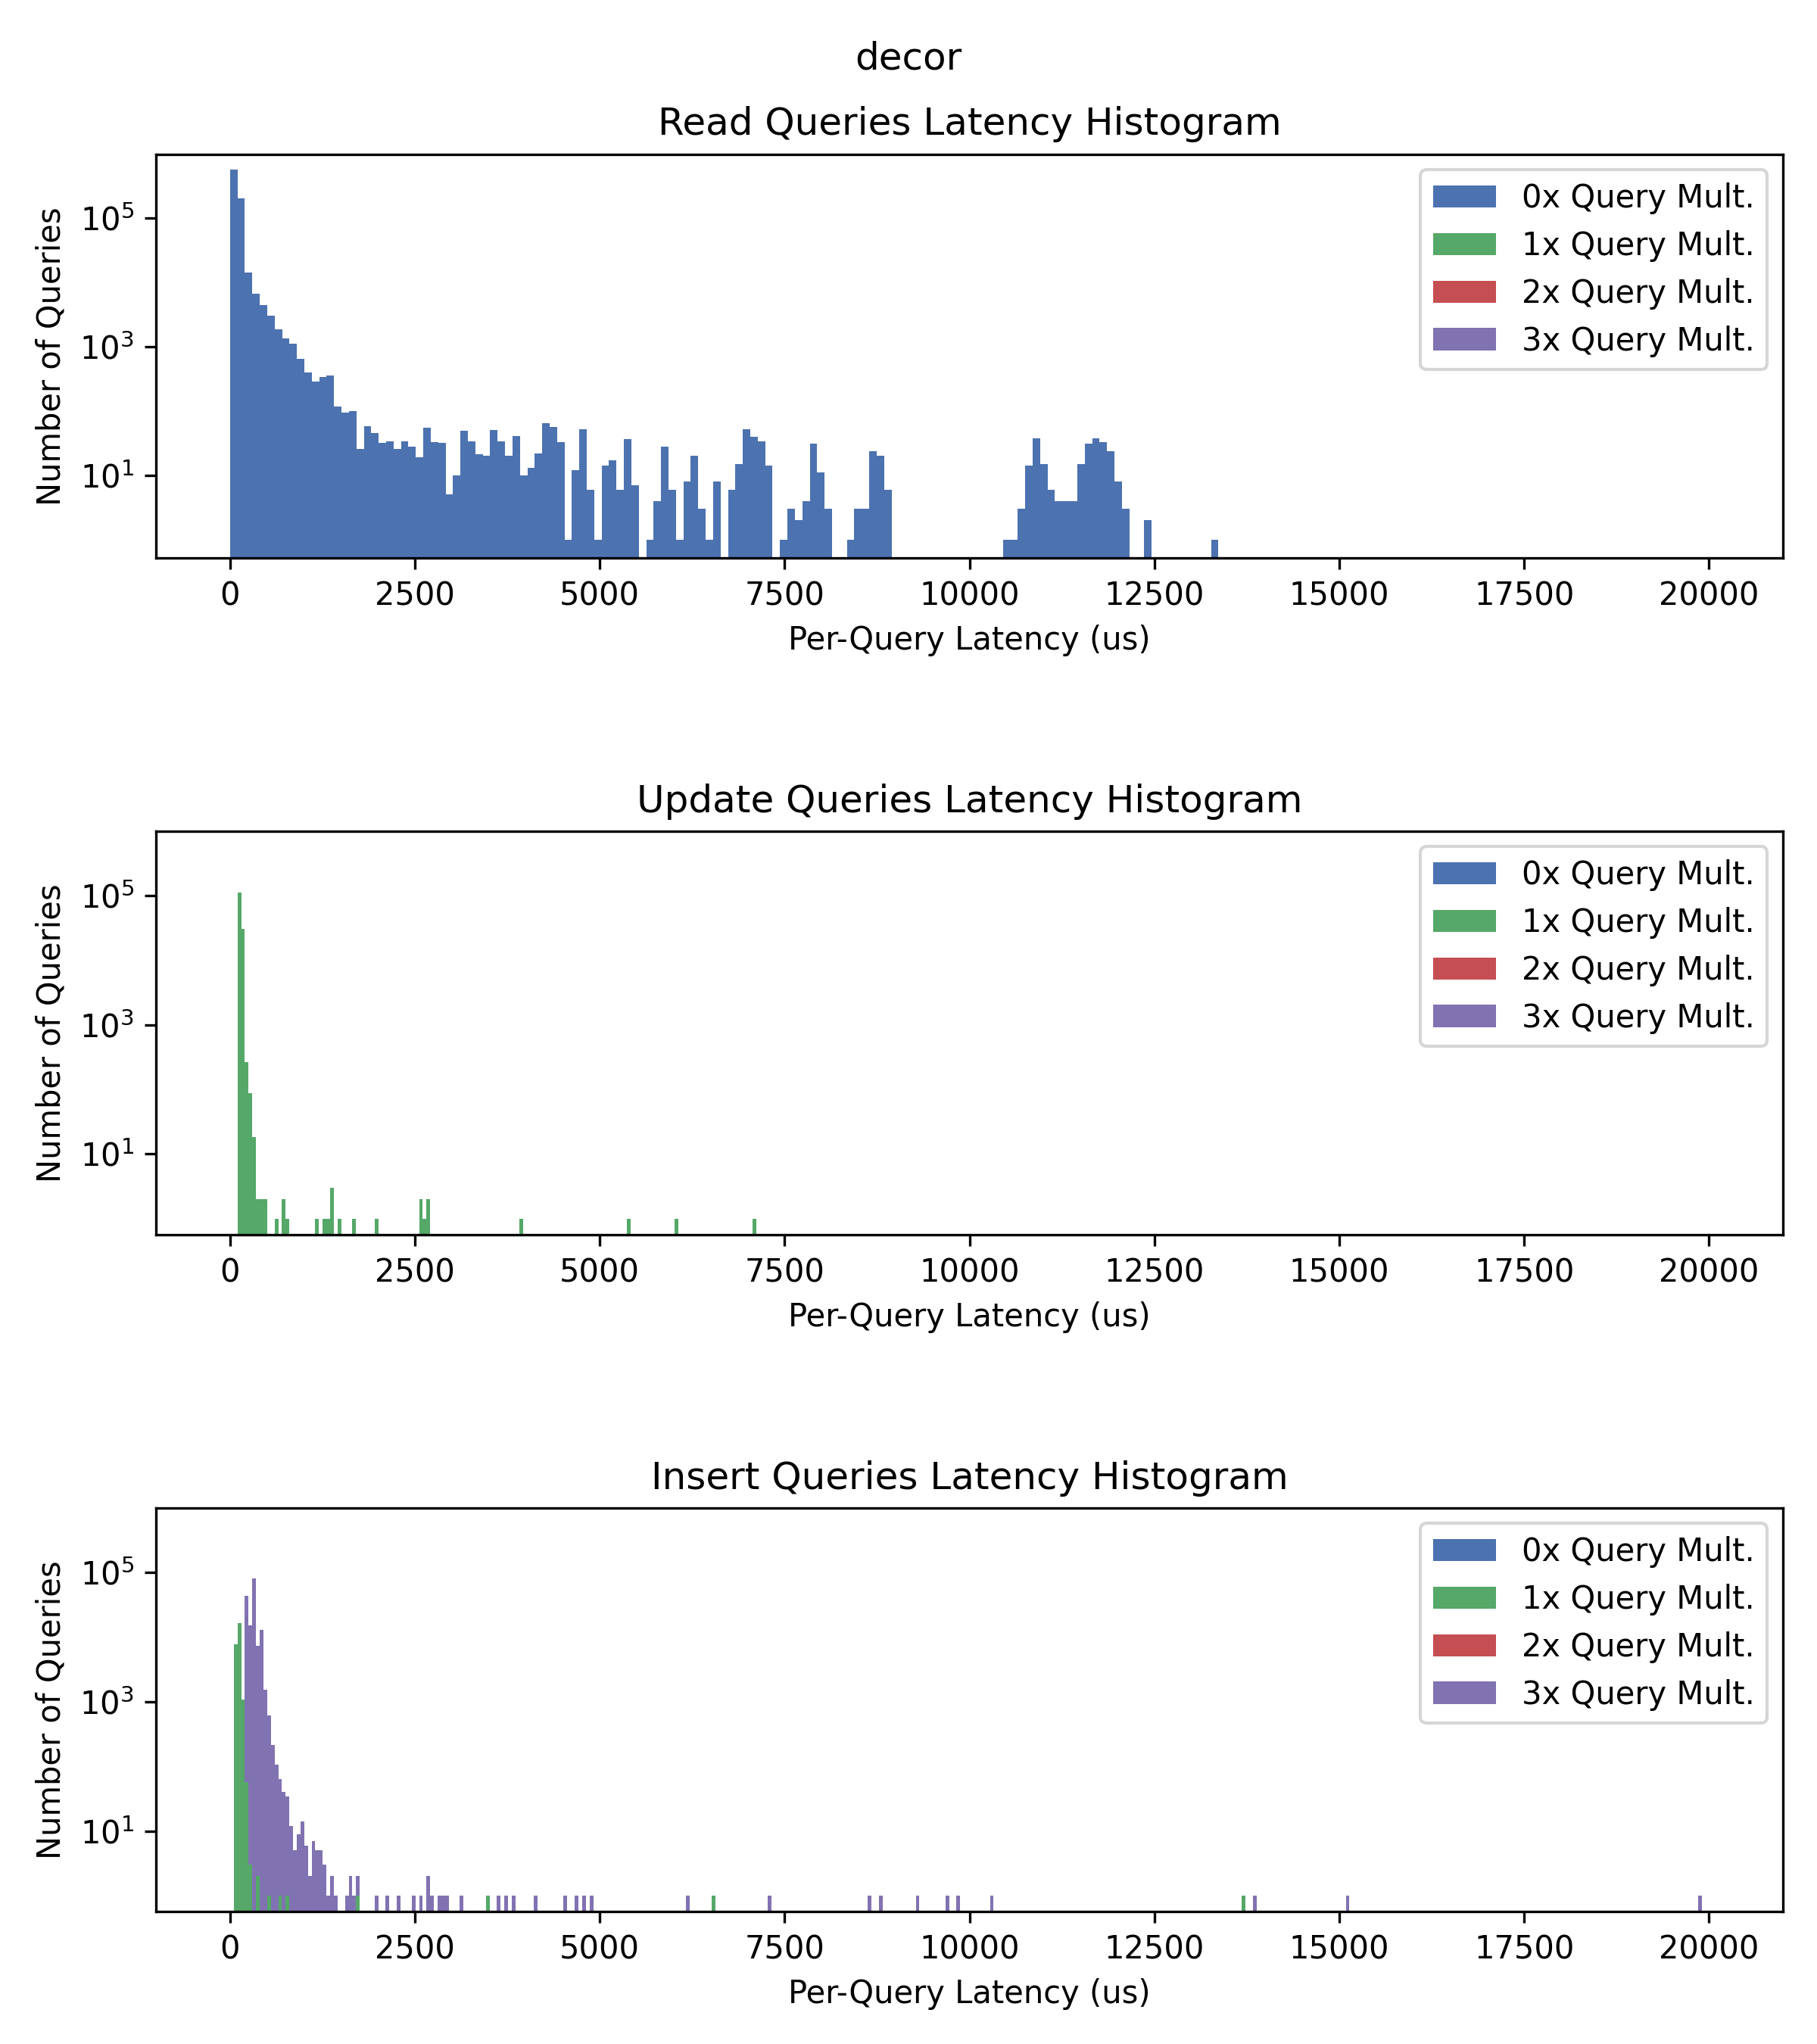
\includegraphics[width=.32\textwidth]{img/decor}
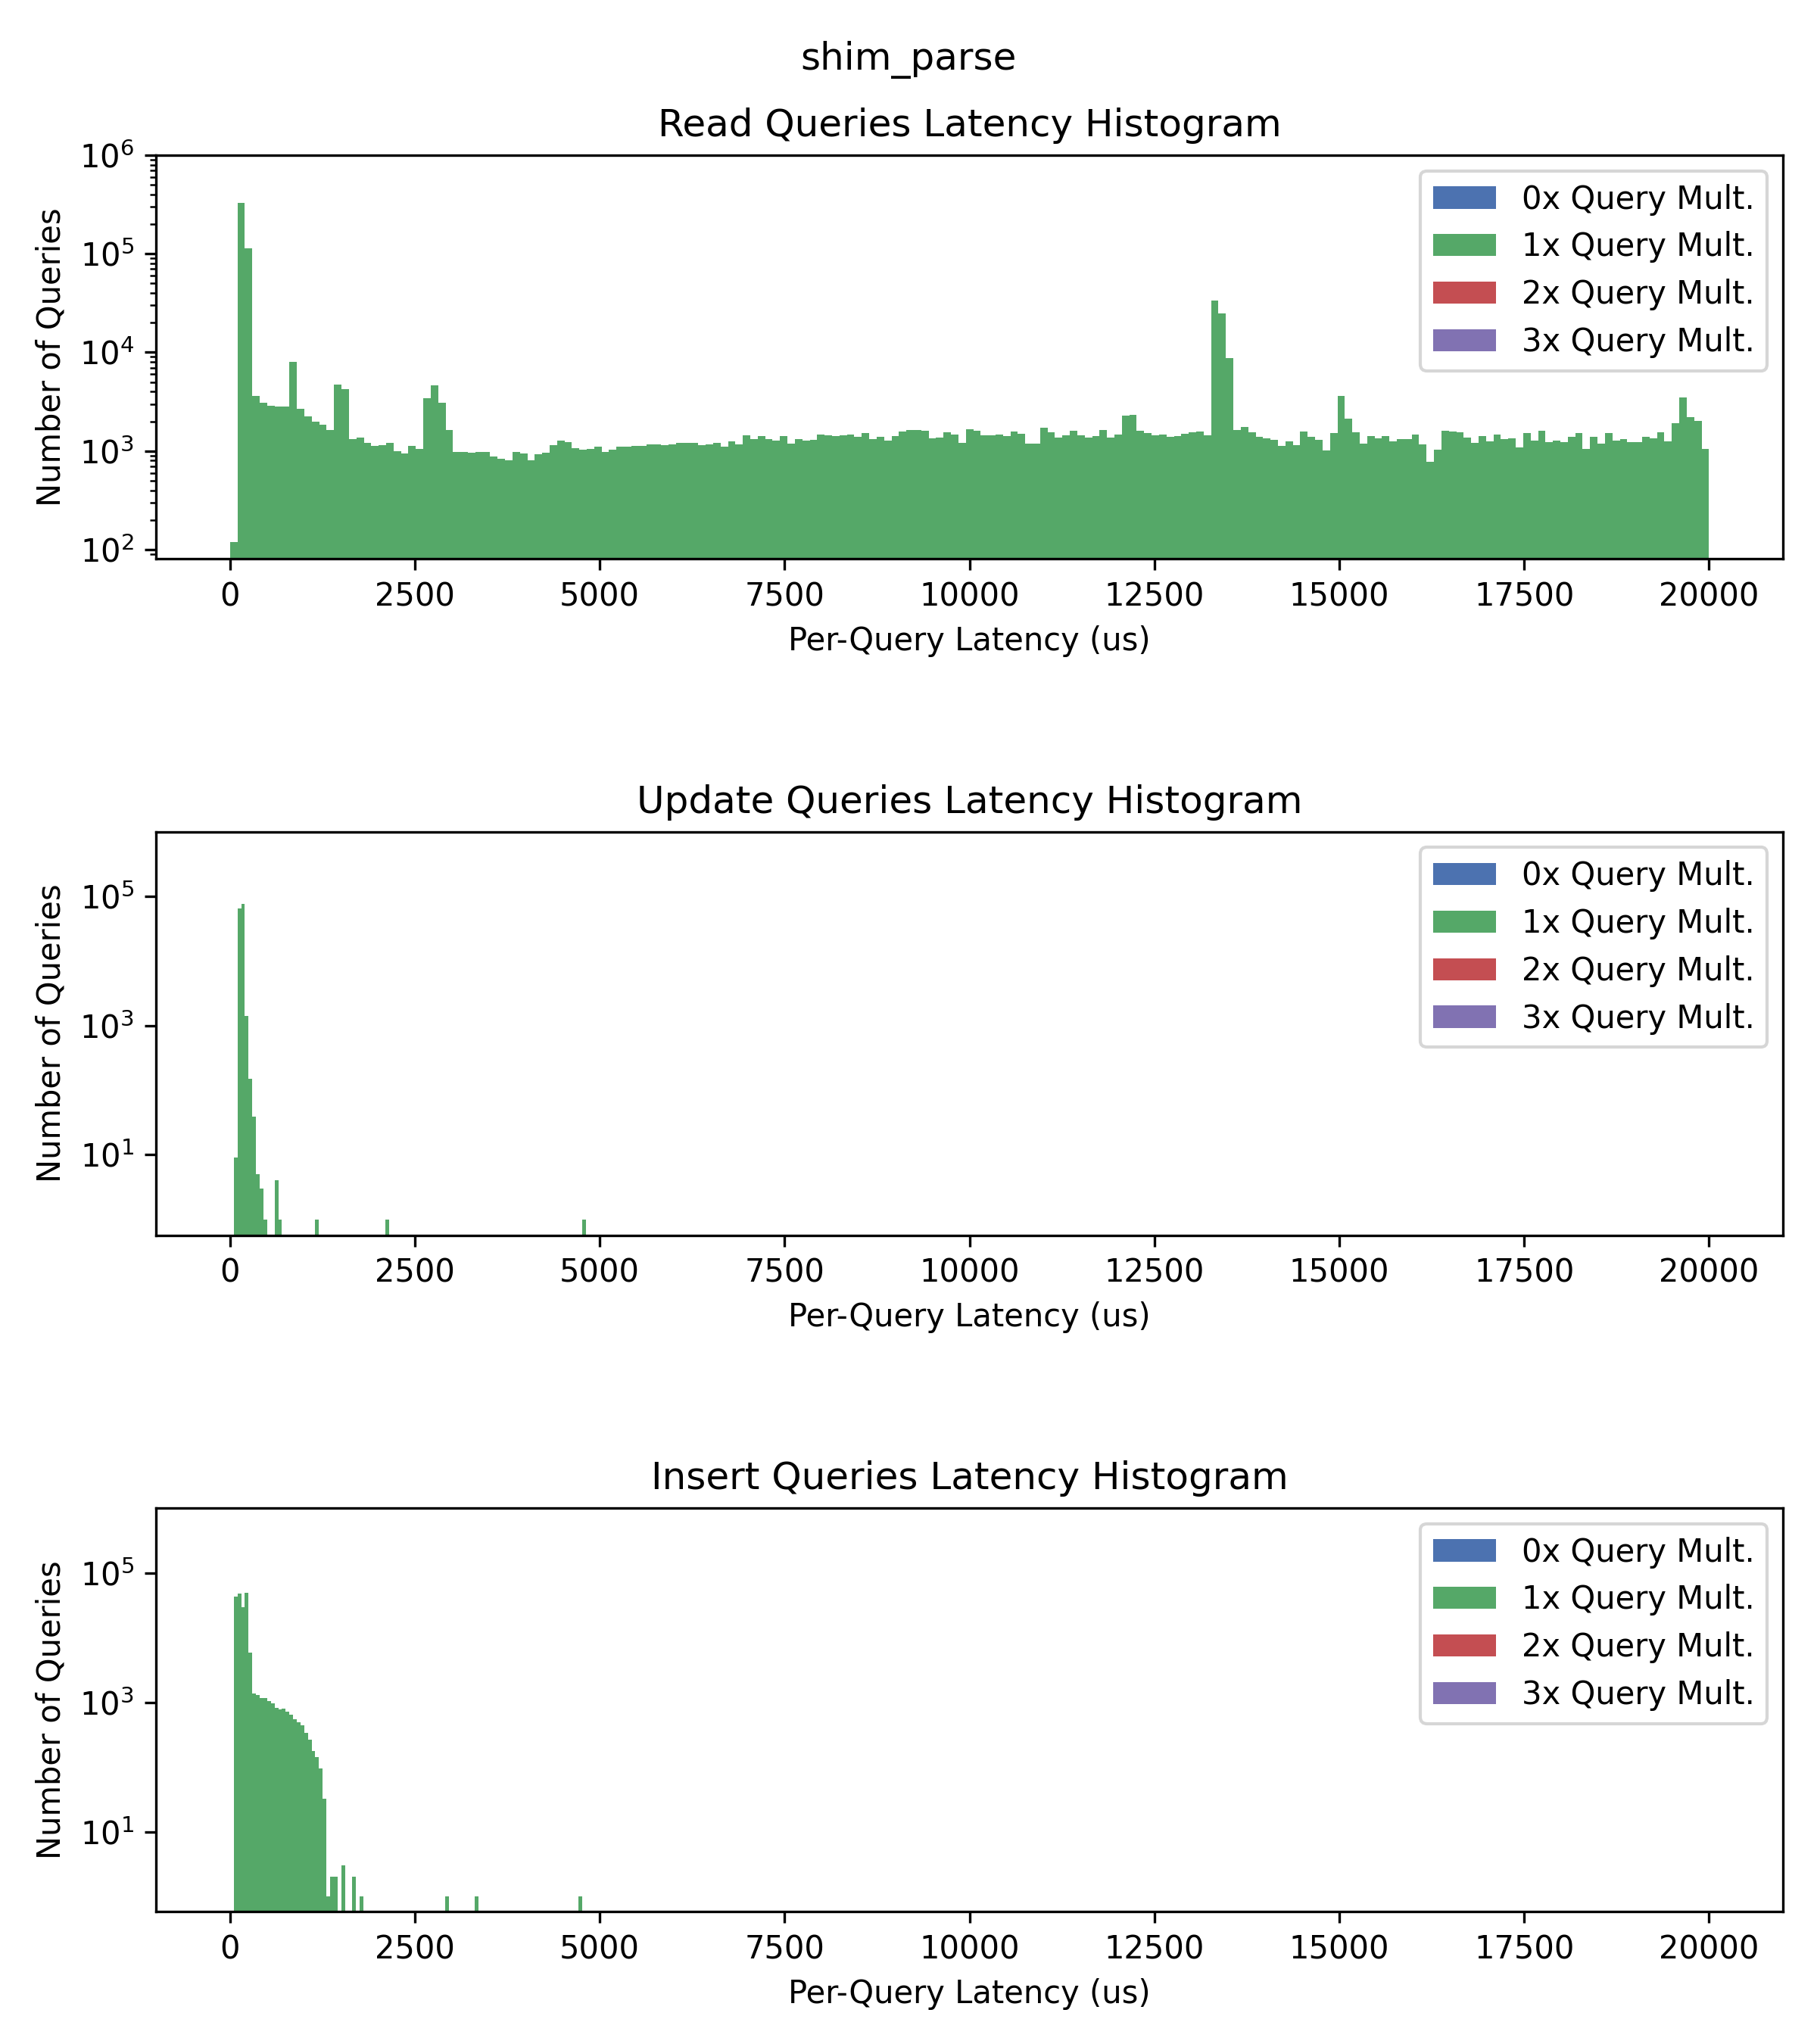
\includegraphics[width=.32\textwidth]{img/shim_parse}
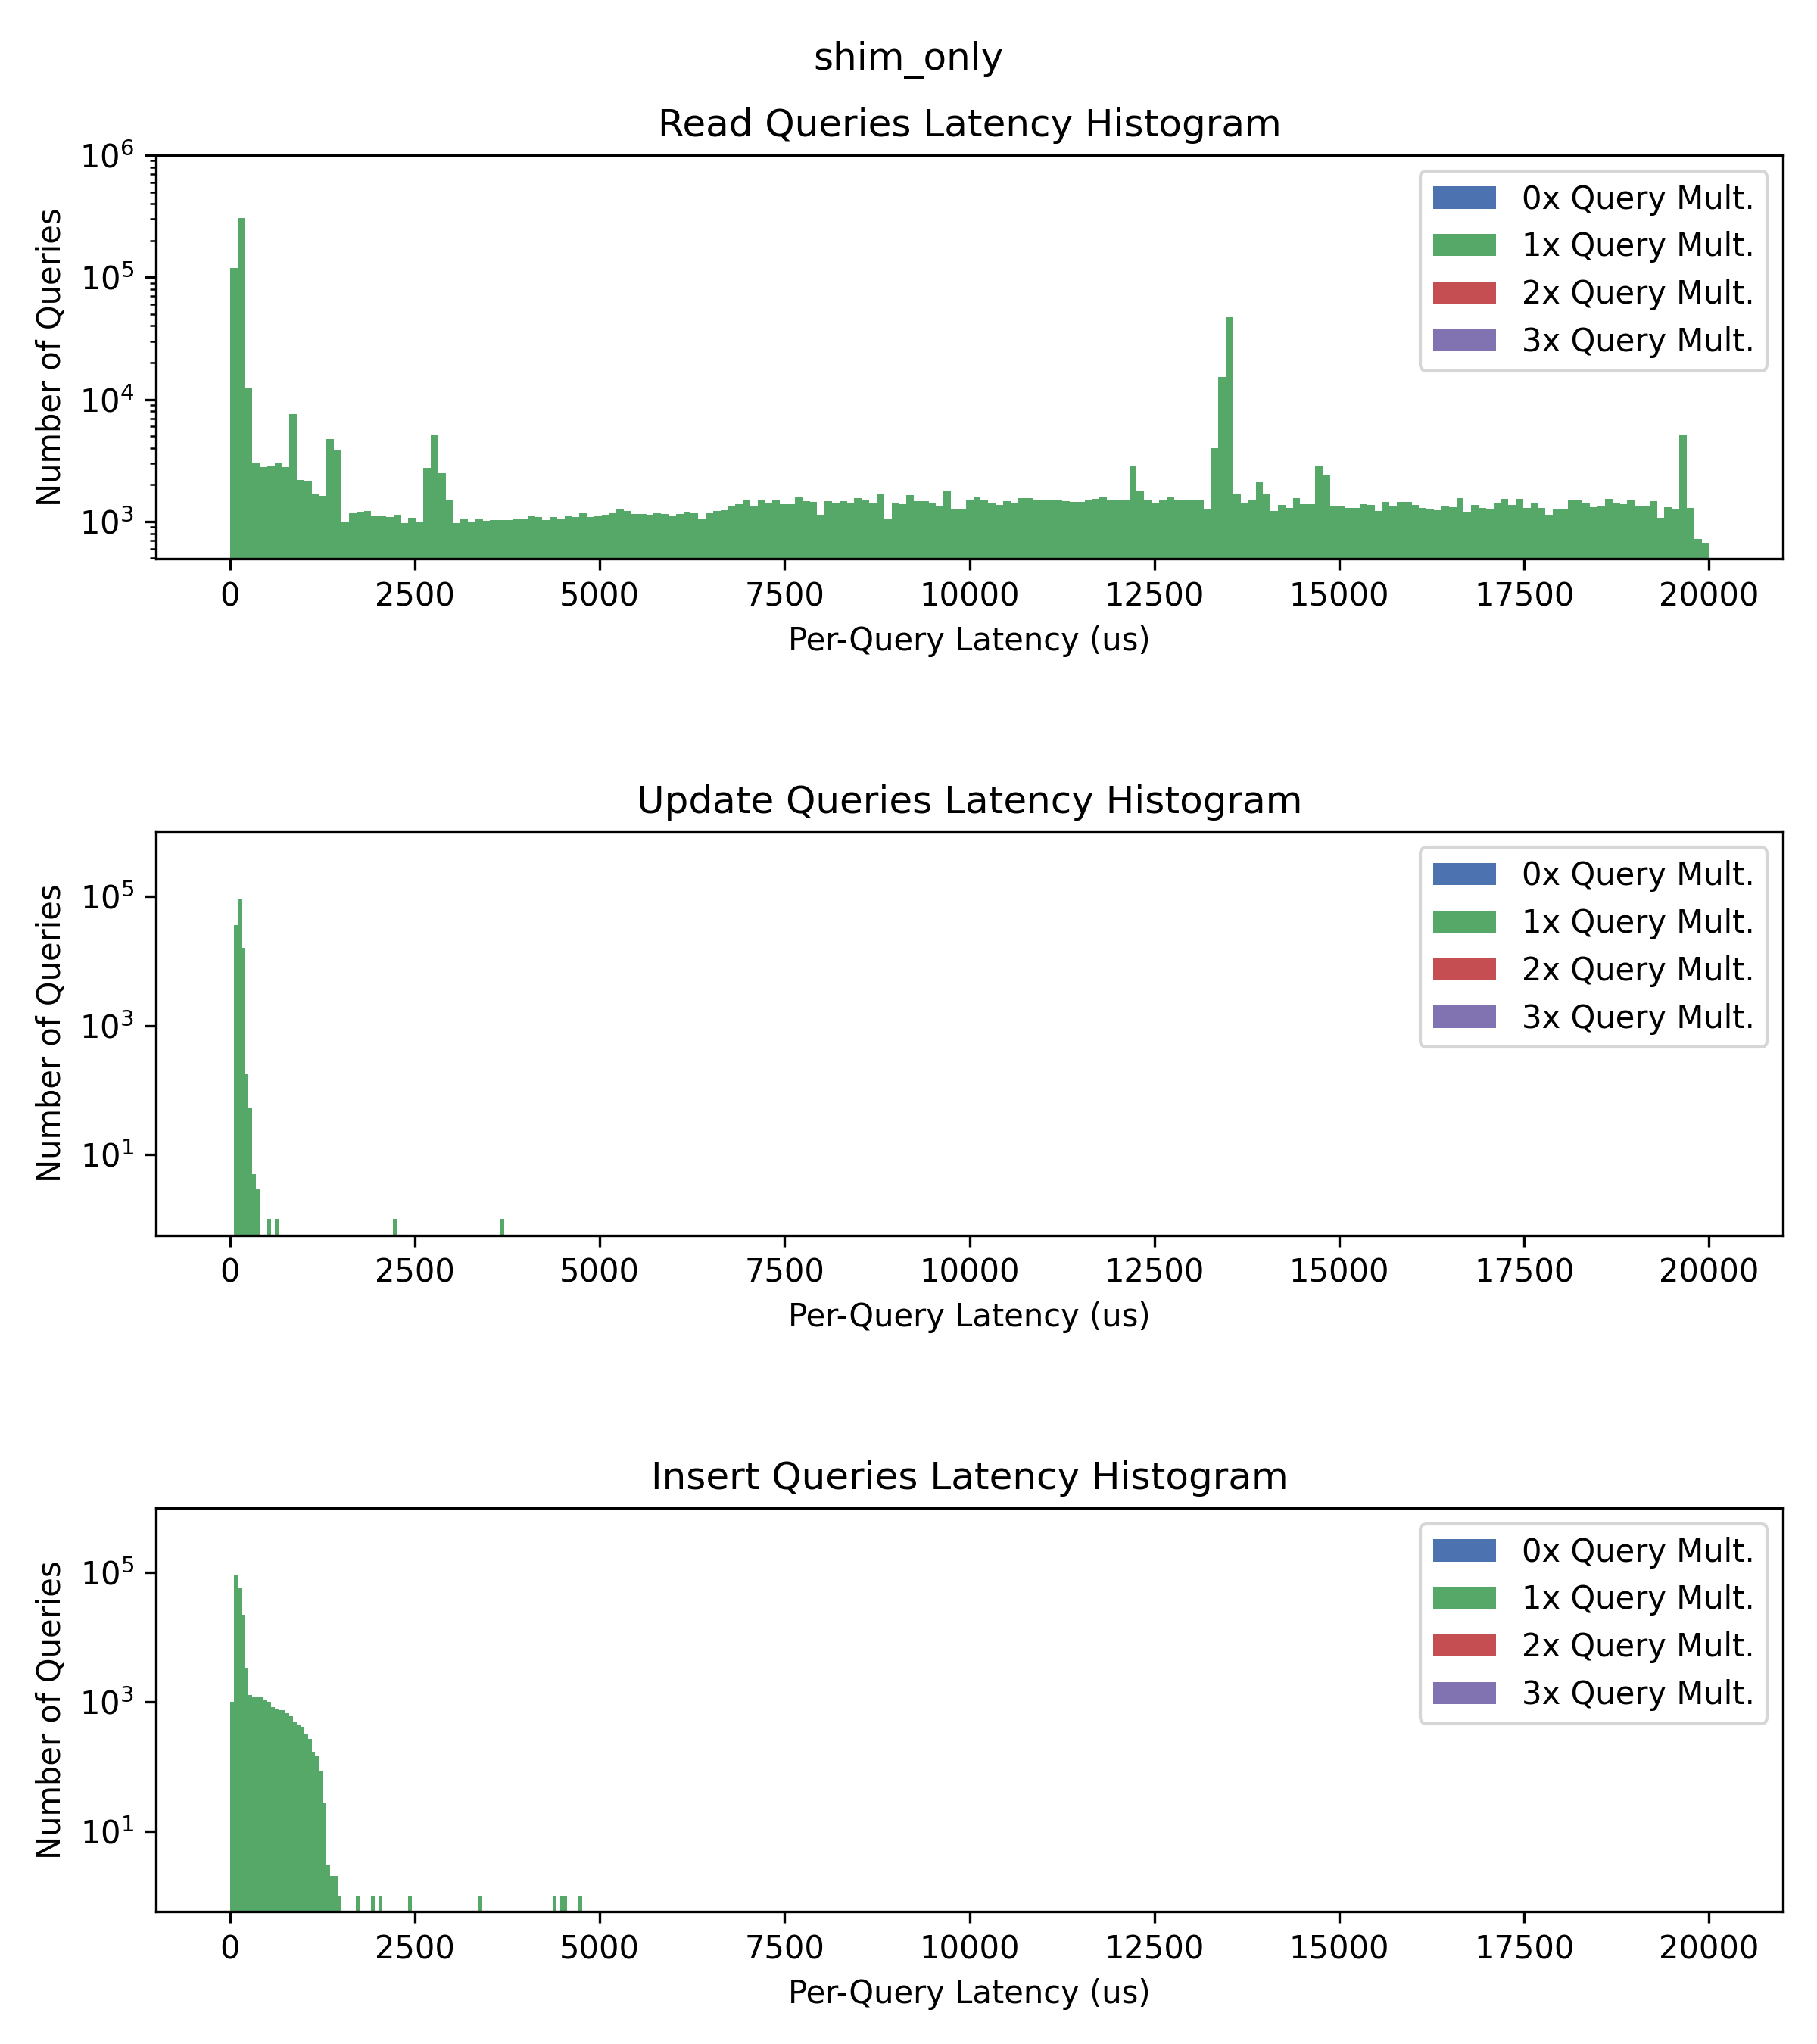
\includegraphics[width=.32\textwidth]{img/shim_only}
    \label{fig:results}
    \caption{Comparison of \sys's latency during normal execution.}
\end{figure*}

\paragraph{Experimental Setup.}
The performance experiments reported are run on Intel Xeon E5-2660 v3 CPUs, with a
single-threaded client and \sys's shim layer each pinned to a single core. \sys runs on top of
MariaDB (v10.4.13).

We compare the application execution performance on four systems, all of which configure MariaDB to
store the database on a ramdisk to avoid disk IO overheads.
\begin{enumerate}
    \item \texttt{NoShim}: queries are directly issued to a MariaDB instance;
    \item \texttt{Shim}: queries are intercepted by the shim layer,
        which does nothing more than send queries to the MariaDB instance and
        return the results back to the client;
    \item \texttt{ShimParsing}: queries are intercepted the shim layer, parsed into a
        SQL AST (which is discarded), and then sent to the MariaDB instance; the shim then returns the results to the
        client.
    \item \texttt{\sys}: queries are intercepted by the shim layer and parsed into a SQL AST. \sys
        then processes the parsed query, potentially introducing ghost entities and sending additional queries to the MariaDB backend.
        \sys then returns results to the client.
\end{enumerate}

We compare \texttt{NoShim} and \texttt{Shim} to define the cost of query interception; \texttt{Shim}
and \texttt{ShimParsing} to define the cost of query parsing; and \texttt{ShimParsing} and
\texttt{\sys} to define the cost of adding decorrelation and recorrelation support.  \texttt{Shim}
provides an upper bound for \sys's (single-threaded) performance, as the costs of query parsing
and decorrelation are not necessarily fundamental.

\paragraph{Lobste.rs Performance}
\sys utilizes the trawler workload~\cite{trawler} for Lobsters, which emulates production
Lobsters traffic according to a recorded production workload. The database initially begins with 3K
users, 20K stories, and 60K comments (1/2 the size of the the real Lobsters deployment), and issues
queries according to the recorded traffic distribution. The query distribution skews towards reads
(recent and frontpage stories) over writes (votes, commenting, and posting of stories); the
workload assumes that users with popular content are also more active and likely to post stories,
comment, and vote.

The benchmarks perform 10000 actions, each performing on average 8 application queries.
We measure (1) overall throughput, (2) the distribution of application query
latencies, (3) the query multiplication per application query performed by \sys, and (4) the
storage cost (in-memory and on-disk).

The first benchmark measures \sys's performance during \emph{normal execution}, namely when only
read and update actions performed by Lobsters are executed.
The second benchmark measures \sys's performance with users unsubscribing 10\% of the time
(approximately 1000 actions are unsubscriptions). If an unsubscribed user is chosen to perform an action, this user is first resubscribed.
\texttt{NoShim}, \texttt{Shim}, and \texttt{ShimParsing} simply delete or insert the chosen user on
unsubscription or resubscription respectively; this provides a very conservative estimate of the
amount of work these baseline systems would need to do if a user withdrew their data from the system.

\lyt{Currently debugging the benchmark... (some error with repeat keys, hopefully won't take too long)}
To complete 10K actions during normal execution, \texttt{NoShim} takes 293s, \texttt{ShimOnly} takes
TODO, \texttt{ShimParse} takes 316s; and \texttt{\sys} takes 185s.
We show the latency results of the second of the Lobsters policies described above in
Figure~\ref{fig:results}.
\lyt{TODO memory usage}
\lyt{Should we also record the amount of time to initialize?}

To complete 10K actions with 10\% of actions being unsubscribe, \texttt{NoShim} takes 263s, \texttt{ShimOnly} takes 277s, \texttt{ShimParse}
takes 284s; and \texttt{\sys} takes TODO.
\lyt{TODO memory usage}
\fi
